\chapter{Method}

This chapter describes the modelling approach used in this thesis. It starts from a simple neural network baseline and then introduces the proposed graph attention network that uses prior gene interactions.

\section{Problem description}
Let $G$ denote the number of genes in the selected gene set. For each perturbation sample, let $x_{\mathrm{ctl}} \in \mathbb{R}^{G}$ be the control profile and $x_{\mathrm{trt}} \in \mathbb{R}^{G}$ be the treatment profile. The supervised target is the response vector
\begin{equation}
y = x_{\mathrm{trt}} - x_{\mathrm{ctl}} \in \mathbb{R}^{G}.
\end{equation}
This formulation focuses on the change after treatment, reduces shared measurement noise between matched control and treatment, and makes responses more comparable across experiments.

\section{Graph neural networks}
A standard neural network typically works on individual data points. It takes a fixed size input vector, which represents features of a single sample, and produces an output. This design works well for many tasks, though it treats each sample as independent. However, in many real world scenarios, data points are connected, both the samples themselves and the links between them carry important information.

A graph neural network (GNN) is designed specifically for such relational data. It models the data as a graph, where nodes represent entities and edges represent the connections between them. At each layer, a node updates its representation by aggregating information from its neighboring nodes. This allows the model to learn from both the features of each node and the structure of the graph itself.

Compared to a standard neural network, this approach offers three practical advantages. First, it uses relational information directly. In a standard network, using graph structure requires manually computing extra features, such as node degree, the number of shared neighbors, or shortest path distances, and adding them to the input. A GNN avoids this preprocessing step. It reads the graph connections directly through its aggregation mechanism and learns relational patterns from start to finish.

Second, the model architecture does not depend on the number of nodes. A standard neural network is designed for a fixed input dimension, so changing the number of nodes often requires redesigning the model. by contrast, A GNN learns a local update rule that applies to any node regardless of the graph's total size. This means the same trained model can be applied to graphs with different numbers of nodes without any architectural changes. 

Third, it is parameter efficient due to shared rules. A standard network often learns separate parameters for each input position. A GNN uses a single shared update function for all nodes. This parameter sharing keeps the total number of trainable parameters relatively low, which often leads to more stable training and better performance when the amount of available data is limited.


The model works in layers. In each layer, a node first collects messages from its neighbours and then updates its own state.
The basic rule is
\begin{equation}
h_{v}^{(\ell+1)} = \sigma\!\left(\sum_{u \in \mathcal{N}(v)} m_{u\rightarrow v}^{(\ell)}\right),
\end{equation}
where $h_{v}^{(\ell)}$ is the state of node $v$ at round $\ell$, and $\mathcal{N}(v)$ is the neighbour set of $v$. In many models, each message $m_{u\rightarrow v}^{(\ell)}$ is computed from the sender state $h_{u}^{(\ell)}$ and the edge between $u$ and $v$. In simple words, each neighbour sends a short message based on its current state; the node adds all incoming messages and then applies a small transform $\sigma(\cdot)$ to get its new state.

The first layer takes the initial node features $h_{v}^{(0)}$ and produces updated features $h_{v}^{(1)}$ that already include information from one hop neighbours. The second layer takes $h_{v}^{(1)}$ and produces $h_{v}^{(2)}$, which now includes information from two hop neighbours, and so on. One layer therefore means a node uses one hop neighbours; two layers mean it can also use two hop neighbours; more layers give a wider view of the graph.

After a small number of layers, the final node states $h_{v}^{(L)}$ are used as learned representations. For node level tasks, a simple output function is applied to each node state to produce one prediction per node. For graph level tasks, the node states are first pooled into a single vector, and then an output function produces one prediction for the whole graph.

\begin{figure}[H]
    \centering
    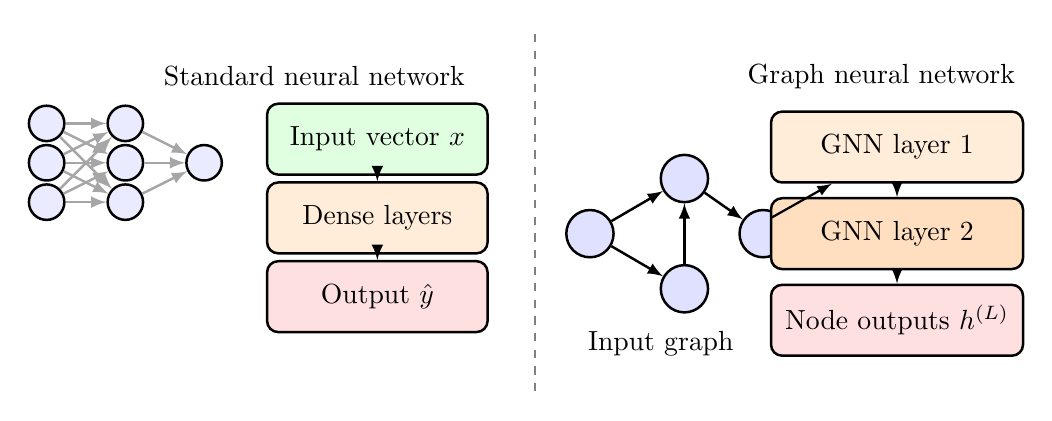
\begin{tikzpicture}[>=latex, line width=0.9pt]
        % Left: standard neural network
        \node[align=center] at (-3.8,3.0) {Standard neural network};

        % Small input nodes (vector view) on the left half
        \node[draw, circle, fill=blue!8, minimum size=0.45cm] (in1) at (-7.2,1.4) {};
        \node[draw, circle, fill=blue!8, minimum size=0.45cm] (in2) at (-7.2,1.9) {};
        \node[draw, circle, fill=blue!8, minimum size=0.45cm] (in3) at (-7.2,2.4) {};

        \node[draw, circle, fill=blue!8, minimum size=0.45cm] (hid1) at (-6.2,1.4) {};
        \node[draw, circle, fill=blue!8, minimum size=0.45cm] (hid2) at (-6.2,1.9) {};
        \node[draw, circle, fill=blue!8, minimum size=0.45cm] (hid3) at (-6.2,2.4) {};

        \node[draw, circle, fill=blue!8, minimum size=0.45cm] (outnode) at (-5.2,1.9) {};

        % Fully connected edges
        \foreach \a in {1,2,3} {
            \foreach \b in {1,2,3} {
                \draw[->, gray!70] (in\a) -- (hid\b);
            }
        }
        \foreach \b in {1,2,3} {
            \draw[->, gray!70] (hid\b) -- (outnode);
        }

        % Box view to the right of the nodes, still on left half
        \node[draw, rounded corners, fill=green!12, minimum width=2.8cm, minimum height=0.9cm] (xvec) at (-3,2.2) {Input vector $x$};
        \node[draw, rounded corners, fill=orange!15, minimum width=2.8cm, minimum height=0.9cm] (dense1) at (-3,1.2) {Dense layers};
        \node[draw, rounded corners, fill=red!12, minimum width=2.8cm, minimum height=0.9cm] (yhat) at (-3,0.2) {Output $\hat{y}$};

        % Arrow from node output to first dense block
        % \draw[->, thick] (outnode) -- (xvec);
        \draw[->] (xvec) -- (dense1);
        \draw[->] (dense1) -- (yhat);

        % Middle separator at x = 0
        \draw[dashed, gray] (-1,-1) -- (-1,3.6);

        % Right: graph neural network
        \node[align=center] at (3.4,3.0) {Graph neural network};

        % Small input graph on the right half (well to the left of the GNN blocks)
        \node[draw, circle, fill=blue!12, minimum size=0.6cm] (v1) at (-0.3,1.0) {};
        \node[draw, circle, fill=blue!12, minimum size=0.6cm] (v2) at (0.9,1.7) {};
        \node[draw, circle, fill=blue!12, minimum size=0.6cm] (v3) at (1.9,1.0) {};
        \node[draw, circle, fill=blue!12, minimum size=0.6cm] (v4) at (0.9,0.3) {};

        \draw[->] (v1) -- (v2);
        \draw[->] (v2) -- (v3);
        \draw[->] (v4) -- (v2);
        \draw[->] (v1) -- (v4);

        \node[align=center] at (0.6,-0.4) {Input graph};

        % Message-passing layers and output (vertical stack)
        \node[draw, rounded corners, fill=orange!15, minimum width=3.2cm, minimum height=0.9cm] (gnn1) at (3.6,2.1) {GNN layer 1};
        \node[draw, rounded corners, fill=orange!25, minimum width=3.2cm, minimum height=0.9cm] (gnn2) at (3.6,1.0) {GNN layer 2};
        \node[draw, rounded corners, fill=red!12, minimum width=3.2cm, minimum height=0.9cm] (gnnout) at (3.6,-0.1) {Node outputs $h^{(L)}$};

        \draw[->, thick] (2.0,1.2) -- (gnn1);
        \draw[->] (gnn1) -- (gnn2);
        \draw[->] (gnn2) -- (gnnout);
    \end{tikzpicture}
    \caption{Comparison between a standard neural network and a graph neural network. Left: a standard network takes a fixed length input vector and processes it through dense layers. Right: a GNN takes a graph as input and uses message passing layers to update node representations before prediction.}
    \label{fig:nn_gnn_comparison}
\end{figure}

\subsection{Graph Convolution Network (GCN)}
GCN is a simple and widely used type of GNN.
A single GCN layer can be described in two steps.
First, each node computes an average of its own features and the features of its neighbours, using a suitable normalization.
Second, this averaged vector is multiplied by a weight matrix and passed through a non-linear function.
In this way, connected nodes can directly influence each other in every layer.

In matrix form, let $A$ be the adjacency matrix that encodes which nodes are connected, $I$ be the identity matrix that adds self connections, $\tilde{A}=A+I$, and $\tilde{D}$ be the degree matrix of $\tilde{A}$. A standard GCN layer is
\begin{equation}
H^{(\ell+1)} = \sigma\!\left(\tilde{D}^{-1/2} \tilde{A}\, \tilde{D}^{-1/2} H^{(\ell)} W^{(\ell)}\right).
\end{equation}
Here $H^{(\ell)}$ stores all node features at round $\ell$, and $W^{(\ell)}$ is a weight matrix learned during training.

A simple example with two GCN layers is
\begin{equation}
H^{(1)} = \mathrm{ReLU}(\hat{A}H^{(0)}W^{(0)}), \qquad
H^{(2)} = \hat{A}H^{(1)}W^{(1)},
\end{equation}
where $\hat{A}=\tilde{D}^{-1/2} \tilde{A}\, \tilde{D}^{-1/2}$.
The first layer takes the initial node features $H^{(0)}$ and produces $H^{(1)}$, which already mixes information from one hop neighbours.
The second layer takes $H^{(1)}$ and produces $H^{(2)}$, which now also reflects information from two hop neighbours.
These final features $H^{(2)}$ are then used to make predictions. Figure~\ref{fig:gnn_practical_example} shows a simple two-layer GCN flow from graph input to output.

\begin{figure}[H]
    \centering
    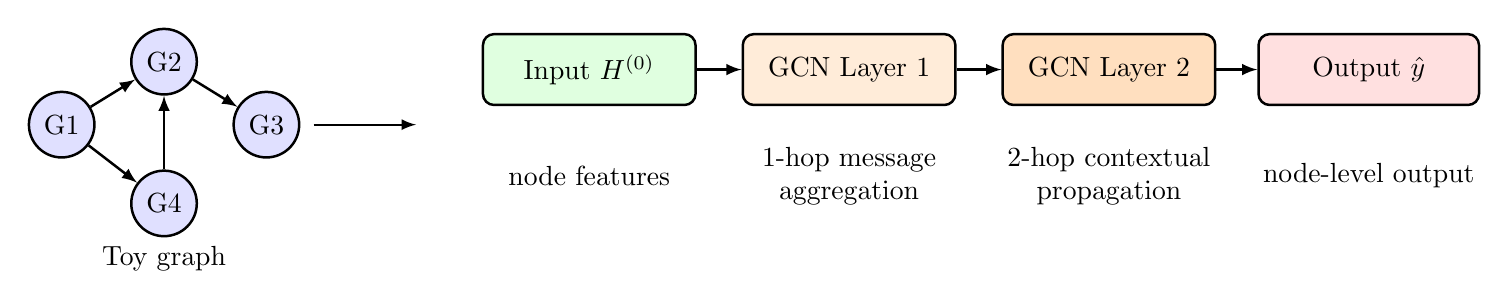
\begin{tikzpicture}[>=latex, line width=0.9pt]
        % Left: toy gene graph
        \node[draw, circle, fill=blue!12, minimum size=0.8cm] (g1) at (0,1.2) {G1};
        \node[draw, circle, fill=blue!12, minimum size=0.8cm] (g2) at (1.3,2.0) {G2};
        \node[draw, circle, fill=blue!12, minimum size=0.8cm] (g3) at (2.6,1.2) {G3};
        \node[draw, circle, fill=blue!12, minimum size=0.8cm] (g4) at (1.3,0.2) {G4};

        \draw[->] (g1) -- (g2);
        \draw[->] (g2) -- (g3);
        \draw[->] (g4) -- (g2);
        \draw[->] (g1) -- (g4);

        \node at (1.3,-0.5) {Toy graph};

        % Middle-right: model pipeline
        \draw[->, thick] (3.2,1.2) -- (4.5,1.2);

        \node[draw, rounded corners, fill=green!12, minimum width=2.7cm, minimum height=0.9cm] (in) at (6.7,1.9) {Input $H^{(0)}$};
        \node[draw, rounded corners, fill=orange!15, minimum width=2.7cm, minimum height=0.9cm] (l1) at (10.0,1.9) {GCN Layer 1};
        \node[draw, rounded corners, fill=orange!25, minimum width=2.7cm, minimum height=0.9cm] (l2) at (13.3,1.9) {GCN Layer 2};
        \node[draw, rounded corners, fill=red!12, minimum width=2.8cm, minimum height=0.9cm] (out) at (16.6,1.9) {Output $\hat{y}$};

        \draw[->] (in) -- (l1);
        \draw[->] (l1) -- (l2);
        \draw[->] (l2) -- (out);

        \node[align=center] at (6.7,0.55) {node features};
        \node[align=center] at (10.0,0.55) {1-hop message\\aggregation};
        \node[align=center] at (13.3,0.55) {2-hop contextual\\propagation};
        \node[align=center] at (16.6,0.55) {node-level output};
    \end{tikzpicture}
    \caption{A practical GNN example: a two-layer GCN. Left: a toy directed graph. Right: computation flow from node features to output features.}
    \label{fig:gnn_practical_example}
\end{figure}
\subsection{Graph Attention Network (GAT)}
GAT extends this idea by learning that different neighbours may have different importance.
In practice, some neighbours provide stronger signals than others, and GAT learns this difference automatically.

For node $v$, the attention weight for neighbour $u$ is
\begin{equation}
\alpha_{u\rightarrow v} = \mathrm{softmax}_{u}\!\left(e_{u\rightarrow v}\right),
\end{equation}
where $e_{u\rightarrow v}$ is a learned score. The update is
\begin{equation}
h_{v}^{(\ell+1)} = \sigma\!\left(\sum_{u \in \mathcal{N}(v)} \alpha_{u\rightarrow v}\, W^{(\ell)} h_{u}^{(\ell)}\right).
\end{equation}
This means useful neighbours get larger weights, and less useful neighbours get smaller weights.
Compared with a standard neural network, this gives a direct way to focus on useful local links.



\begin{figure}[H]
    \centering
    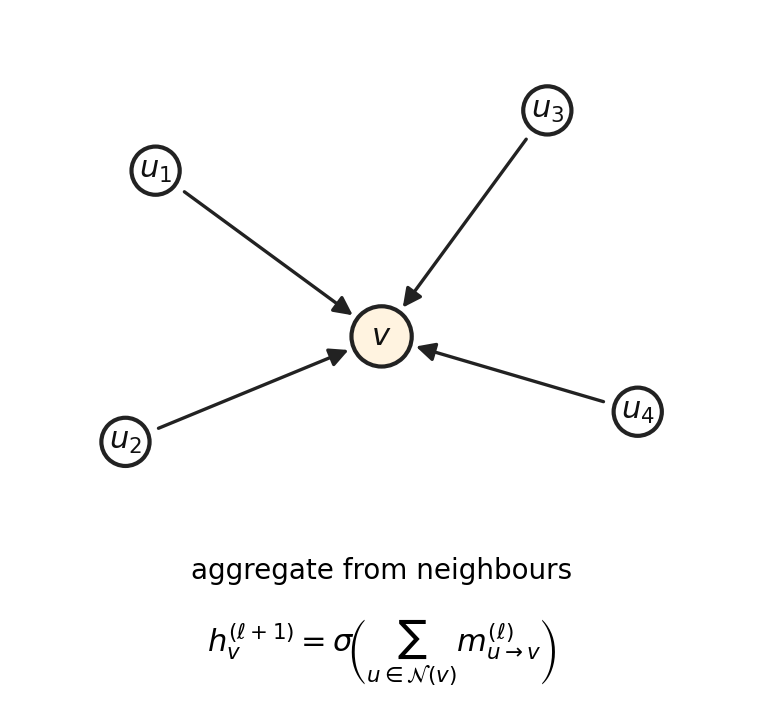
\includegraphics[width=0.75\linewidth]{figures/gnn_message_passing.png}
    \caption{Message passing in a GNN. The representation of a node $v$ is updated by aggregating information from its neighbours.}
    \label{fig:gnn_message_passing}
\end{figure}

\begin{figure}[H]
    \centering
    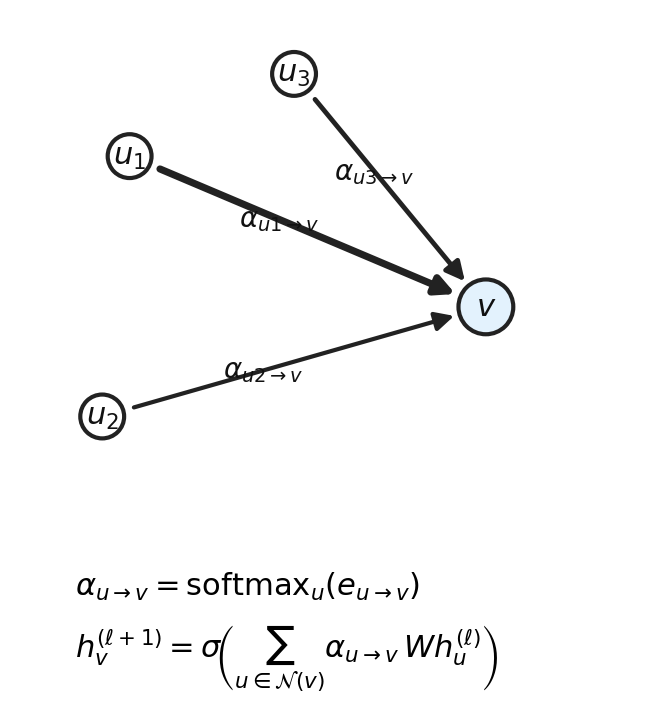
\includegraphics[width=0.75\linewidth]{figures/gat_attention.png}
    \caption{GAT update idea. Neighbours send messages to the same target node $v$, and the model learns different weights $\alpha_{u\rightarrow v}$ for different neighbours.}
    \label{fig:gat_attention}
\end{figure}

\section{Baseline model}
As a non-graph baseline, we use a standard neural network that predicts $\hat{y}$ from the control profile and drug features. This baseline shows how much can be learned without any explicit gene interaction structure.

\subsection{Inputs}
The baseline model uses:
\begin{enumerate}
\item the control expression profile $x_{\mathrm{ctl}}$;
\item drug targets encoded as a sparse vector aligned to the gene list;
\item a molecular fingerprint as a fixed-length drug descriptor.
\end{enumerate}

\subsection{Architecture and output}
The inputs are concatenated and passed through several fully connected layers to produce the predicted response vector $\hat{y} \in \mathbb{R}^{G}$.

\section{Proposed model}
\subsection{Graph construction}
Prior biological knowledge is represented as a directed graph $\mathcal{G}=(\mathcal{V},\mathcal{E})$ built from OmniPath. Nodes correspond to genes in the selected gene set. Edges represent known regulator-to-target or interaction relationships. When available, interaction type is encoded as a signed edge weight $w_{uv}\in\{+1,-1\}$.

\subsection{Model inputs and node features}
The proposed model uses one node per gene. Node features are initialized from the control profile:
\begin{equation}
H^{(0)} = \phi(x_{\mathrm{ctl}}) \in \mathbb{R}^{G \times F},
\end{equation}
where $\phi(\cdot)$ maps each scalar expression value to an $F$-dimensional feature vector. Drug targets are represented as a sparse vector aligned to the same gene order and injected as an additional input signal. Drug fingerprints provide a dense drug representation that conditions the model on chemical structure.

\subsection{GAT backbone}
The model uses $L$ graph attention layers to propagate information over $\mathcal{G}$. Attention weights determine how strongly each neighbour contributes to the update, following the mechanism described in the previous section. Signed edge weights $w_{uv}$ are used when available to encode activating or inhibiting relations.

\subsection{Prediction head}
After $L$ layers, a per-node readout produces the predicted response vector $\hat{y}\in\mathbb{R}^{G}$.

\section{Training}
\subsection{Loss function}
Training minimizes a regression loss between $y$ and $\hat{y}$. A gene mask is applied when only a subset of genes should contribute to the loss. The objective combines a mean squared error term with a correlation term based on the Pearson correlation coefficient at the sample level.

\subsection{Counterfactual drug loss}
To check that the model uses drug information, counterfactual inputs are created by modifying drug features while keeping the same control profile and cell context. Two modes are used: \emph{zero} sets drug features to zero, and \emph{shuffle} assigns drug features from another sample in the same batch. A margin-based hinge penalty is applied when the counterfactual loss is too close to the factual loss. This encourages factual predictions to be better than counterfactual predictions by a fixed margin.

\section{Evaluation and interpretation}
Generalization is evaluated under cold drug and cold cell splits. Performance is reported using sample-wise PCC and MSE. Attention weights are used as an interpretation signal by aggregating edge attentions across samples, and by grouping attentions by drug or by cell line when needed.
